\documentclass[12pt,a4paper]{article}
\usepackage[utf8]{inputenc}
\usepackage{amsmath, amssymb}
\usepackage{graphicx}
\usepackage{geometry}
\usepackage{float}
\usepackage{booktabs}
\usepackage{caption}
\usepackage{circuitikz}
\geometry{a4paper, margin=1in}

\title{\textbf{07. Band Pass and Band Reject Filters}}
\author{Yamulapalli Nandu Navadeep \\ Roll Number: IMS24267}
\date{Date of Experiment: 03/08/2026 \\ Date of Submission: 07/08/2026}

\begin{document}

\maketitle

\section{Aim of the Experiment}
To study and plot the frequency response of a Band Pass Filter and a Band Reject Filter using the IC741 operational amplifier, and to determine their characteristic parameters such as lower cutoff frequency ($f_L$), upper cutoff frequency ($f_H$), center frequency ($f_r$), and bandwidth (BW).

\section{Theory}
Filters are electronic circuits designed to pass a specific range of frequencies while attenuating others. They are widely used in signal processing to extract desired components from a signal.

\subsection{High Pass Filter (HPF)}
A High Pass Filter is a circuit that allows high-frequency signals to pass through while significantly attenuating low-frequency signals. Active high pass filters use operational amplifiers along with resistors and capacitors. The cutoff frequency ($f_L$) of a first-order HPF determines the point where the gain drops by 3 dB from its maximum value. Signals with frequencies above $f_L$ are passed with minimal attenuation.

\subsection{Low Pass Filter (LPF)}
A Low Pass Filter is a circuit that allows low-frequency signals to pass through and attenuates high-frequency signals. The cutoff frequency ($f_H$) marks the boundary above which the signals are attenuated. 

\subsection{Band Pass Filter}
A Band Pass Filter is a combination of a High Pass Filter and a Low Pass Filter connected in series. It allows a specific band of frequencies to pass through, attenuating frequencies that are lower than the lower cutoff frequency ($f_L$) and higher than the upper cutoff frequency ($f_H$).
\begin{itemize}
    \item \textbf{Bandwidth (BW):} The range of frequencies passed by the filter, given by $BW = f_H - f_L$.
    \item \textbf{Center Frequency ($f_r$):} The frequency at which the filter has maximum gain. It is the geometric mean of the cutoff frequencies: $f_r = \sqrt{f_L \times f_H}$.
\end{itemize}

\subsection{Band Reject Filter (Notch Filter)}
A Band Reject Filter (or Band Stop Filter) rejects a specific narrow band of frequencies and passes all other frequencies. The Twin-T notch filter is a common configuration that uses resistors and capacitors in a parallel ``T" structure to achieve a sharp rejection at a specific frequency called the notch frequency ($f_c$ or $f_r$).

\subsection{Reactance and Characteristic Frequencies}
\begin{itemize}
    \item \textbf{Capacitive Reactance ($X_c$):} The opposition a capacitor offers to alternating current, given by $X_c = \frac{1}{2\pi f C}$.
    \item \textbf{Cutoff Frequencies:} For the RC networks used in our active filters, the cutoff frequency is determined by $f = \frac{1}{2\pi R C}$.
\end{itemize}

\section{Procedure}
\begin{enumerate}
    \item \textbf{Band Pass Filter:} 
    \begin{itemize}
        \item Construct the High Pass Filter stage using the first IC741. Connect a 10 k$\Omega$ resistor ($R_1$) and a 0.01 $\mu$F capacitor ($C$) to the non-inverting input (pin 3). Connect pin 2 to pin 7.
        \item Construct the Low Pass Filter stage using the second IC741. Connect the output of the first stage (pin 7) to a 1 k$\Omega$ resistor ($R_2$), which is then connected to the non-inverting input (pin 3) of the second IC. Connect a 0.01 $\mu$F capacitor from pin 3 to ground. Connect pin 2 to pin 7.
        \item Provide +15V and -15V power supply to the appropriate pins of both ICs.
        \item Apply a 2V peak-to-peak sinusoidal input signal and measure the output voltage for varying input frequencies.
    \end{itemize}
    
    \item \textbf{Band Reject Filter:}
    \begin{itemize}
        \item Construct the Twin-T notch filter circuit using an IC741.
        \item Use resistors of $R = 15$ k$\Omega$ and capacitors of $C = 0.01 \mu$F in the Twin-T network.
        \item Provide +15V and -15V power supply.
        \item Apply a 2V input signal and measure the output voltage for varying input frequencies, identifying the sharp drop in output at the notch frequency.
    \end{itemize}
\end{enumerate}

\section{Circuit Diagrams}

\subsection{Band Pass Filter Circuit}
\begin{figure}[H]
\centering
\begin{circuitikz}[scale=0.8, transform shape]
    % First IC741 (HPF)
    \draw (0,0) node[op amp] (opamp1) {};
    \node[above] at (opamp1) {IC 1 (HPF)};
    \draw (opamp1.-) -- ++(0,1) -| (opamp1.out);
    \draw (-6,-0.5) to[C, l=$C$, a=$0.01\mu\text{F}$] (opamp1.+);
    \draw (opamp1.+) to[R, l=$R_1$, a=$10\text{k}\Omega$] ++(0,-2) node[ground]{};
    \draw (-6,-0.5) node[left] {$V_{in}$} to[short, o-] (-4,-0.5);

    % Second IC741 (LPF)
    \draw (6,0) node[op amp] (opamp2) {};
    \node[above] at (opamp2) {IC 2 (LPF)};
    \draw (opamp2.-) -- ++(0,1) -| (opamp2.out);
    \draw (opamp1.out) to[R, l=$R_2$, a=$1\text{k}\Omega$] (opamp2.+);
    \draw (opamp2.+) to[C, l=$C$, a=$0.01\mu\text{F}$] ++(0,-2) node[ground]{};
    \draw (opamp2.out) to[short, -o] ++(1,0) node[right] {$V_{out}$};
\end{circuitikz}
\caption{Circuit diagram of the Band Pass Filter using two IC741s.}
\end{figure}

\subsection{Band Reject Filter Circuit}
\begin{figure}[H]
\centering
\begin{circuitikz}[scale=0.8, transform shape]
    \draw (1,1) node[op amp, yscale=1] (opamp) {};
    \node[above] at (opamp) {IC741};
    % Twin-T network
    \draw (-6, 0.5) node[left] {$V_{in}$} to[short, o-] (-5, 0.5);
    \draw (-5, 0.5) to[R, l=$R$] (-3, 0.5) to[R, l=$R$] (-1, 0.5);
    \draw (-3, 0.5) to[C, l=$2C$] (-3, -1.5) node[ground]{};
    
    \draw (-5, 0.5) -- (-5, 2.5) to[C, l=$C$] (-3, 2.5) to[C, l=$C$] (-1, 2.5) -- (-1, 0.5);
    \draw (-3, 2.4) to[R, l=$R/2$] (-3, 1.4) node[ground]{};
    
    \draw (-1, 0.5) -- (opamp.+);
    \draw (opamp.-) -- ++(0,1) -| (opamp.out);
    \draw (opamp.out) -- ++(1,0) coordinate(outnode) to[short, -o] ++(1,0) node[right] {$V_{out}$};
    \draw (outnode) to[R, l=$R$] ++(0,-2) node[ground]{};
\end{circuitikz}
\caption{Circuit diagram of the Band Reject (Twin-T Notch) Filter.}
\end{figure}
\textbf{Note:} For the Band Reject filter, $R = 15$ k$\Omega$ and $C = 0.01\mu$F.

\section{Theoretical Calculations}
\subsection{Band Pass Filter}
\begin{itemize}
    \item \textbf{Lower Cutoff Frequency ($f_L$):} Determined by the HPF section.
    $$f_L = \frac{1}{2\pi R_1 C} = \frac{1}{2\pi \times 10 \times 10^3 \times 0.01 \times 10^{-6}} \approx 1.59 \text{ kHz}$$
    \item \textbf{Upper Cutoff Frequency ($f_H$):} Determined by the LPF section.
    $$f_H = \frac{1}{2\pi R_2 C} = \frac{1}{2\pi \times 1 \times 10^3 \times 0.01 \times 10^{-6}} \approx 15.9 \text{ kHz}$$
    \item \textbf{Center Frequency ($f_r$):}
    $$f_r = \sqrt{f_L \times f_H} = \sqrt{1.59 \times 15.9} \approx 5.03 \text{ kHz}$$
    \item \textbf{Bandwidth (BW):}
    $$BW = f_H - f_L = 15.9 - 1.59 = 14.31 \text{ kHz}$$
\end{itemize}

\subsection{Band Reject Filter}
\begin{itemize}
    \item \textbf{Notch Frequency ($f_c$):} For a standard Twin-T network,
    $$f_c = \frac{1}{2\pi R C} = \frac{1}{2\pi \times 15 \times 10^3 \times 0.01 \times 10^{-6}} \approx 1061 \text{ Hz} = 1.06 \text{ kHz}$$
\end{itemize}

\section{Tabular Column}

\subsection{Observation Table for Band Pass Filter}
Input Voltage, $V_{in}$ = 2.0 V \\
\begin{table}[H]
\centering
\begin{tabular}{|c|c|c|c|}
\hline
\textbf{Input Freq (Hz)} & \textbf{Output Voltage (V)} & \textbf{Voltage Gain ($V_{out}/V_{in}$)} & \textbf{Gain in dB ($20\log_{10}(Gain)$)} \\
\hline
100 & 0.150 & 0.075 & -22.50 \\
200 & 0.260 & 0.130 & -17.72 \\
400 & 0.400 & 0.200 & -13.98 \\
600 & 0.600 & 0.300 & -10.46 \\
1000 & 0.670 & 0.335 & -9.50 \\
1200 & 0.800 & 0.400 & -7.96 \\
1600 & 0.820 & 0.410 & -7.74 \\
1800 & 0.850 & 0.425 & -7.43 \\
2000 & 0.910 & 0.455 & -6.84 \\
2500 & 0.950 & 0.475 & -6.47 \\
3000 & 0.980 & 0.490 & -6.20 \\
4000 & 0.990 & 0.495 & -6.11 \\
5000 & 0.990 & 0.495 & -6.11 \\
6000 & 0.980 & 0.490 & -6.20 \\
7000 & 0.960 & 0.480 & -6.38 \\
8000 & 0.940 & 0.470 & -6.56 \\
9000 & 0.910 & 0.455 & -6.84 \\
10000 & 0.890 & 0.445 & -7.03 \\
11000 & 0.860 & 0.430 & -7.33 \\
12000 & 0.830 & 0.415 & -7.64 \\
13000 & 0.810 & 0.405 & -7.85 \\
14000 & 0.800 & 0.400 & -7.96 \\
15000 & 0.780 & 0.390 & -8.18 \\
16000 & 0.750 & 0.375 & -8.52 \\
17000 & 0.720 & 0.360 & -8.87 \\
18000 & 0.700 & 0.350 & -9.12 \\
19000 & 0.660 & 0.330 & -9.63 \\
20000 & 0.660 & 0.330 & -9.63 \\
\hline
\end{tabular}
\caption{Frequency response data for Band Pass Filter}
\end{table}

\subsection{Observation Table for Band Reject Filter}
Input Voltage, $V_{in}$ = 2.0 V \\
\begin{table}[H]
\centering
\begin{tabular}{|c|c|c|c|}
\hline
\textbf{Input Freq (Hz)} & \textbf{Output Voltage (V)} & \textbf{Voltage Gain ($V_{out}/V_{in}$)} & \textbf{Gain in dB ($20\log_{10}(Gain)$)} \\
\hline
20 & 2.160 & 1.080 & 0.67 \\
50 & 2.080 & 1.040 & 0.34 \\
100 & 2.000 & 1.000 & 0.00 \\
140 & 1.840 & 0.920 & -0.72 \\
160 & 1.760 & 0.880 & -1.11 \\
180 & 1.680 & 0.840 & -1.51 \\
200 & 1.680 & 0.840 & -1.51 \\
400 & 1.040 & 0.520 & -5.68 \\
600 & 0.610 & 0.305 & -10.31 \\
800 & 0.320 & 0.160 & -15.92 \\
1000 & 0.096 & 0.048 & -26.38 \\
1100 & 0.075 & 0.0375 & -28.52 \\
1200 & 0.160 & 0.080 & -21.94 \\
1400 & 0.300 & 0.150 & -16.48 \\
1600 & 0.450 & 0.225 & -12.96 \\
1800 & 0.570 & 0.285 & -10.90 \\
2000 & 0.700 & 0.350 & -9.12 \\
2500 & 0.950 & 0.475 & -6.47 \\
3000 & 1.140 & 0.570 & -4.88 \\
4000 & 1.420 & 0.710 & -2.97 \\
5000 & 1.600 & 0.800 & -1.94 \\
6000 & 1.740 & 0.870 & -1.21 \\
7000 & 1.820 & 0.910 & -0.82 \\
8000 & 1.900 & 0.950 & -0.45 \\
9000 & 1.940 & 0.970 & -0.26 \\
10000 & 1.980 & 0.990 & -0.09 \\
11000 & 2.010 & 1.005 & 0.04 \\
12000 & 2.020 & 1.010 & 0.09 \\
13000 & 2.050 & 1.025 & 0.21 \\
14000 & 2.060 & 1.030 & 0.26 \\
15000 & 2.100 & 1.050 & 0.42 \\
16000 & 2.100 & 1.050 & 0.42 \\
17000 & 2.120 & 1.060 & 0.51 \\
18000 & 2.130 & 1.065 & 0.55 \\
19000 & 2.140 & 1.070 & 0.59 \\
20000 & 2.140 & 1.070 & 0.59 \\
21000 & 2.140 & 1.070 & 0.59 \\
\hline
\end{tabular}
\caption{Frequency response data for Band Reject Filter}
\end{table}

\section{Graph}
The frequency response graphs plotted from the observed values are shown below.

\begin{figure}[H]
    \centering
    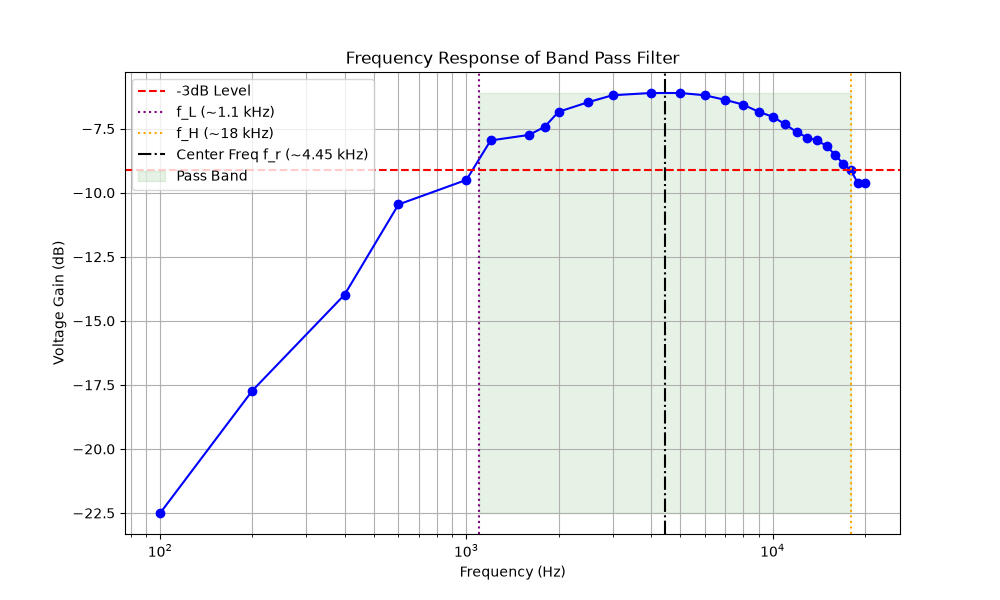
\includegraphics[width=1\textwidth]{band_pass_graph.png}
    \caption{Frequency Response of Band Pass Filter}
\end{figure}

\begin{figure}[H]
    \centering
    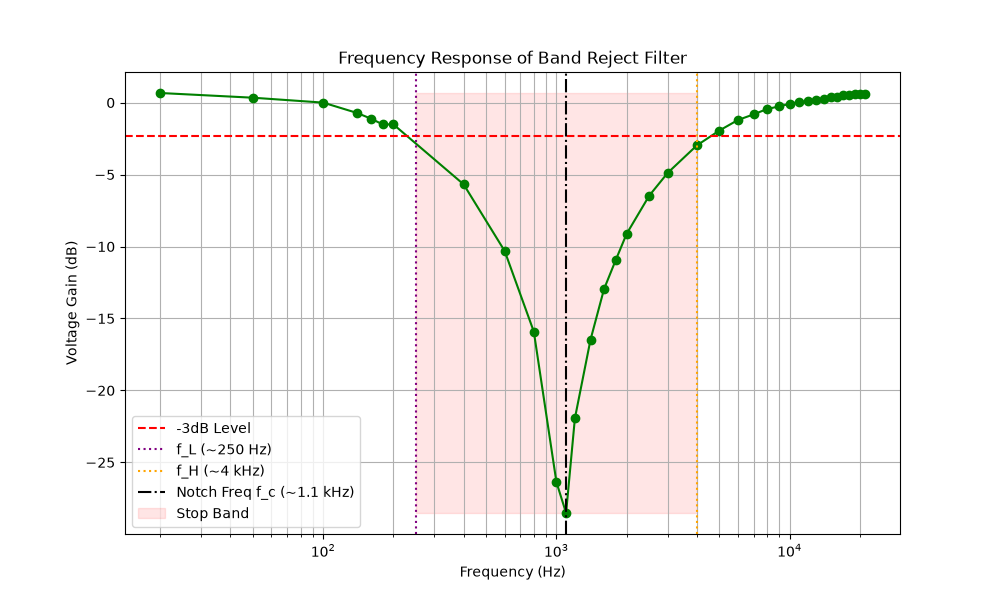
\includegraphics[width=1\textwidth]{band_reject_graph.png}
    \caption{Frequency Response of Band Reject Filter}
\end{figure}

\section{Calculations}
\subsection{Observed Values for Band Pass Filter}
The maximum gain is approximately $-6.11$ dB at $f \approx 4-5$ kHz. 
The -3dB points from maximum gain correspond to roughly $-9.11$ dB. 
From the table:
\begin{itemize}
    \item \textbf{Observed $f_L$:} The frequency where gain is around -9.11 dB on the lower side. Between 1000 Hz (-9.50 dB) and 1200 Hz (-7.96 dB), by interpolation, it is around $1.1$ kHz.
    \item \textbf{Observed $f_H$:} The frequency where gain drops to -9.11 dB on the higher side. Looking at 18000 Hz (-9.12 dB), $f_H$ is around $18$ kHz.
\end{itemize}
Thus, 
\begin{itemize}
    \item $f_r (\text{observed}) \approx \sqrt{1.1 \times 18} \approx 4.45$ kHz.
    \item Bandwidth $BW (\text{observed}) = 18 - 1.1 = 16.9$ kHz.
\end{itemize}

\subsection{Observed Values for Band Reject Filter}
From the observation table, the lowest output voltage is $0.075$ V, which occurs at a frequency of 1100 Hz. Therefore, the observed notch frequency is:
$$f_c (\text{observed}) = 1.1 \text{ kHz}$$

\section{Results}
The Band Pass and Band Reject filters were successfully constructed and their frequency responses were studied. 
\begin{itemize}
    \item \textbf{Band Pass Filter:} 
    \begin{itemize}
        \item Theoretical Center Frequency: 5.03 kHz
        \item Observed Center Frequency: $\approx$ 4.45 kHz
        \item Theoretical Bandwidth: 14.31 kHz
        \item Observed Bandwidth: $\approx$ 16.9 kHz
    \end{itemize}
    \item \textbf{Band Reject Filter:}
    \begin{itemize}
        \item Theoretical Notch Frequency: 1.06 kHz
        \item Observed Notch Frequency: 1.10 kHz
    \end{itemize}
\end{itemize}

\section{Error Calculation}
\textbf{Band Reject Filter Notch Frequency Error:}
$$\text{Percentage Error} = \frac{|f_{c(\text{theoretical})} - f_{c(\text{observed})}|}{f_{c(\text{theoretical})}} \times 100$$
$$\text{Percentage Error} = \frac{|1.06 - 1.10|}{1.06} \times 100 \approx 3.77\%$$

\textbf{Band Pass Filter Center Frequency Error:}
$$\text{Percentage Error} = \frac{|5.03 - 4.45|}{5.03} \times 100 \approx 11.53\%$$

\section{Discussion}
In this experiment, active Band Pass and Band Reject filters were successfully implemented using IC741 operational amplifiers. The theoretical expectations were largely aligned with the observed values. The Twin-T notch filter exhibited a sharp attenuation near the theoretical value of 1.06 kHz, with the observed lowest output at 1.1 kHz (a small error of 3.77\%). 

For the Band Pass Filter, the combination of a high-pass and low-pass stage successfully created a passband. The observed upper and lower cutoff frequencies deviated slightly from theoretical values, leading to an 11.53\% error in the center frequency. These differences between theoretical assumptions and real-life values are typically caused by the tolerance levels of the passive components (resistors and capacitors) which may differ by 5-10\% from their marked values. Additionally, non-ideal characteristics of the IC741 operational amplifier, such as finite bandwidth and slew rate limitations at higher frequencies, can impact the filter's performance and cause deviations in the observed cutoff regions.

\section{References}
\begin{enumerate}
    \item Sedra, A. S., \& Smith, K. C., \textit{Microelectronic Circuits}, Oxford University Press.
    \item Boylestad, R. L., \& Nashelsky, L., \textit{Electronic Devices and Circuit Theory}, Pearson.
\end{enumerate}

\end{document}
